\documentclass[a4paper]{exam}
\usepackage[margin=1in]{geometry}
\usepackage{amsmath}
\usepackage{geometry}
\usepackage{tikz}
% \usetikzlibrary{graphviz}
\usetikzlibrary{backgrounds}

\tikzstyle{arrow} = [->,>=stealth]
\tikzstyle{node} = [auto,font=\footnotesize,draw,circle]

\printanswers
\begin{document}
\begin{center}
{\Large \textbf{Spring 2024}}\vspace{1.0em}\\
{\Large \textbf{CS 412 (Algorithms: Design and Analysis)}}\vspace{1.0em}\\
{\Large \textbf{Weekly Challenge 06: Graph Algorithms}}\vspace{1.0em}\\
{\Large Announced: Friday, February 23, 2024.}\\
\vspace{.25em}
{\Large Deadline: Friday, March 1, 2024 (11:59 pm PKT).}\\ 
\vspace{.3em}
{\Large Total marks: 1.}
\vspace{.5em}\\
\end{center}
\textbf{Instructions}: Submit \textbf{individually} your solution as a PDF with the file name as your $studentID.pdf$; typeset in LaTeX. You must submit your solution on Canvas.

\centerline{\rule{.7\textwidth}{1pt}}
\begin{questions}
\question[1]
  Consider the graph, $\mathcal{G}$, below with 10 nodes and 13 edges. 
  \begin{center}
    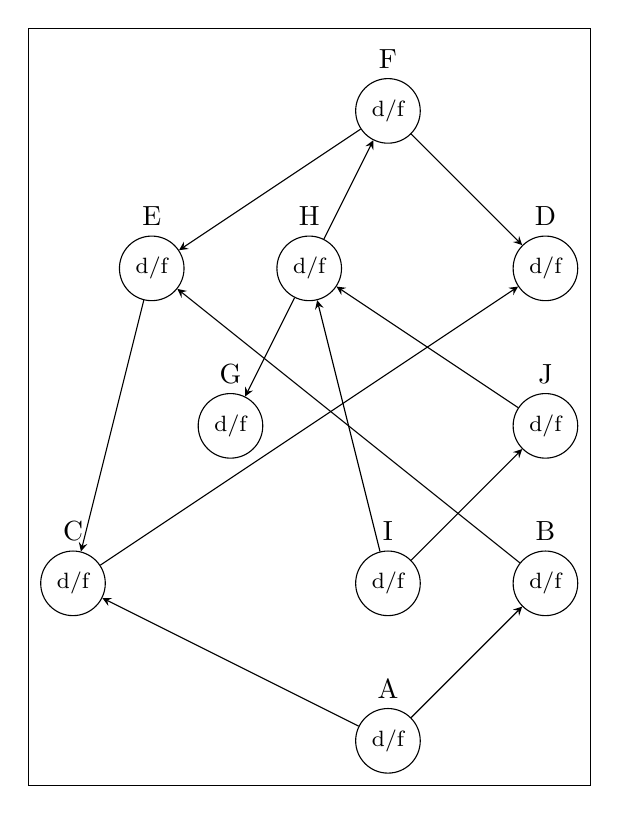
\begin{tikzpicture}[show background rectangle]
      \node[node] [anchor=north, label={A}] (a) at (5, 1) {d/f};
      \node[node] [anchor=north, label={B}] (b) at (7, 3) {d/f};
      \node[node] [anchor=north, label={C}] (c) at (1, 3) {d/f};
      \node[node] [anchor=north, label={D}] (d) at (7, 7) {d/f};
      \node[node] [anchor=north, label={E}] (e) at (2, 7) {d/f};
      \node[node] [anchor=north, label={F}] (f) at (5, 9) {d/f};
      \node[node] [anchor=north, label={G}] (g) at (3, 5) {d/f};
      \node[node] [anchor=north, label={H}] (h) at (4, 7) {d/f};
      \node[node] [anchor=north, label={I}] (i) at (5, 3) {d/f};
      \node[node] [anchor=north, label={J}] (j) at (7, 5) {d/f};

      \draw[arrow] (a) -- (c);
      \draw[arrow] (c) -- (d);
      \draw[arrow] (f) -- (d);
      \draw[arrow] (f) -- (e);
      \draw[arrow] (e) -- (c);
      \draw[arrow] (a) -- (b);
      \draw[arrow] (b) -- (e);
      \draw[arrow] (h) -- (f);
      \draw[arrow] (h) -- (g);
      \draw[arrow] (j) -- (h);
      \draw[arrow] (i) -- (h);
      \draw[arrow] (i) -- (j);
    \end{tikzpicture}
  \end{center}
  The procedure, $\text{DFS}(\mathcal{G})$, is executed on the graph such that ties are resolved in alphabetical order.
  \begin{parts}
  \part Redraw the graph below such that each node, $n$, contains $n.d/n.f$, where $n.d$ and $n.f$ are the node's discovery and finalization times respectively. Mention your starting nodes/nodes under the graph.
  \part Draw below the corresponding DFS-forest.
  \end{parts}
  
  \begin{solution}
    \begin{parts}
      \part Starting the DFS from node $A$, and after that, we begin by node $I$
      \begin{center}
        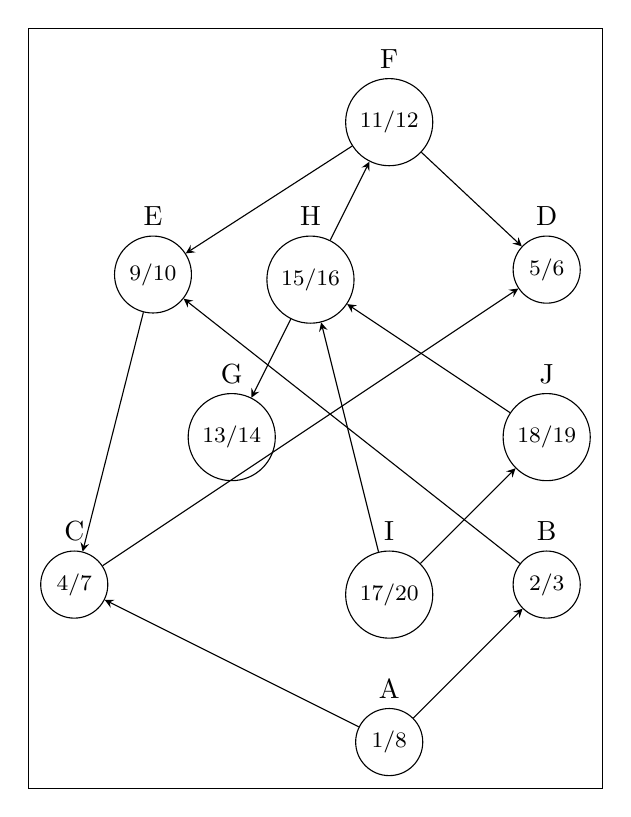
\begin{tikzpicture}[show background rectangle]
          \node[node] [anchor=north, label={A}] (a) at (5, 1) {1/8};
          \node[node] [anchor=north, label={B}] (b) at (7, 3) {2/3};
          \node[node] [anchor=north, label={C}] (c) at (1, 3) {4/7};
          \node[node] [anchor=north, label={D}] (d) at (7, 7) {5/6};
          \node[node] [anchor=north, label={E}] (e) at (2, 7) {9/10};
          \node[node] [anchor=north, label={F}] (f) at (5, 9) {11/12};
          \node[node] [anchor=north, label={G}] (g) at (3, 5) {13/14};
          \node[node] [anchor=north, label={H}] (h) at (4, 7) {15/16};
          \node[node] [anchor=north, label={I}] (i) at (5, 3) {17/20};
          \node[node] [anchor=north, label={J}] (j) at (7, 5) {18/19};
    
          \draw[arrow] (a) -- (c);
          \draw[arrow] (c) -- (d);
          \draw[arrow] (f) -- (d);
          \draw[arrow] (f) -- (e);
          \draw[arrow] (e) -- (c);
          \draw[arrow] (a) -- (b);
          \draw[arrow] (b) -- (e);
          \draw[arrow] (h) -- (f);
          \draw[arrow] (h) -- (g);
          \draw[arrow] (j) -- (h);
          \draw[arrow] (i) -- (h);
          \draw[arrow] (i) -- (j);
        \end{tikzpicture}
      \end{center}
      
      \part The below DFS-forest correspond to part(a)
      
      % \begin{tikzpicture}[level distance=1.5cm, sibling distance=2cm,
      %   every node/.style={circle,draw}]
        
      %   \node (A) {A}
      %     child {node (B) {B}
      %       child {node (E) {E}
      %         child {node (C) {C}
      %           child {node (D) {D}}
      %         }
      %       }
      %     };
          
      %   % DFS edges
      %   \draw (A) -- (B);
      %   \draw (B) -- (E);
      %   \draw (E) -- (C);
      %   \draw (C) -- (D);
        
      % \end{tikzpicture}

      % \begin{tikzpicture}[level distance=1.5cm, sibling distance=2cm,
      %   every node/.style={circle,draw}]
        
      %   \node (I) {I}
      %     child {node (J) {J}
      %       child {node (H) {H}
      %         child {node (F) {F}}
      %         child {node (G) {G}}
      %       }
      %     };
          
      %   % DFS edges
      %   \draw (I) -- (J);
      %   \draw (J) -- (H);
      %   \draw (H) -- (F);
      %   \draw (H) -- (G);
        
      % \end{tikzpicture}

      % A (B C (D) ) 
      % E 
      % F 
      % G
      % H 
      % I J
      \noindent
      \begin{minipage}[t]{0.45\textwidth}
      \centering
      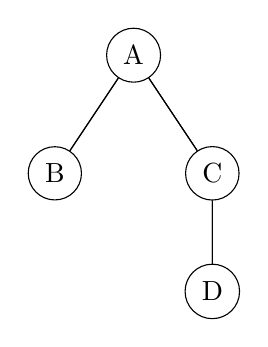
\begin{tikzpicture}[level distance=1.5cm, sibling distance=2cm,
        every node/.style={circle,draw}]
        
        \node (A) {A}
          child {node (B) {B}}
            child {node (C) {C}
              child {node (D) {D}}
            }
          ;
          
        % DFS edges
        \draw (A) -- (B);
        \draw (A) -- (C);
        \draw (C) -- (D);

        
      \end{tikzpicture}
      \end{minipage}
      \hfill
      \begin{minipage}[t]{0.35\textwidth}
      \centering
      
\begin{tikzpicture}[level distance=1.5cm, sibling distance=2cm,
        every node/.style={circle,draw}]
        
        \node (E) {E};
        
      \end{tikzpicture}
      \end{minipage}
      \hfill
      \begin{minipage}[t]{0.35\textwidth}
      \centering
      
\begin{tikzpicture}[level distance=1.5cm, sibling distance=2cm,
        every node/.style={circle,draw}]
        
        \node (F) {F};
        
      \end{tikzpicture}
      \end{minipage}
      \hfill
      \begin{minipage}[t]{0.45\textwidth}
      \centering
      
\begin{tikzpicture}[level distance=1.5cm, sibling distance=2cm,
        every node/.style={circle,draw}]
        
        \node (G) {G};
        
      \end{tikzpicture}
      \end{minipage}
      \hfill
      \begin{minipage}[t]{0.45\textwidth}
      \centering
      
\begin{tikzpicture}[level distance=1.5cm, sibling distance=2cm,
        every node/.style={circle,draw}]
        
        \node (H) {H};
        
      \end{tikzpicture}
      \end{minipage}

      \hfill
      \begin{minipage}[t]{0.45\textwidth}
      \centering
      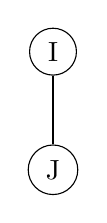
\begin{tikzpicture}[level distance=1.5cm, sibling distance=2cm,
        every node/.style={circle,draw}]
        
        \node (I) {I}
          child {node (J) {J}};
          
        % DFS edges
        \draw (I) -- (J);
        
      \end{tikzpicture}
      \end{minipage}

      % % \hfill
      % \begin{minipage}[t]{0.45\textwidth}
      % \centering
      % \begin{tikzpicture}[level distance=1.5cm, sibling distance=2cm,
      %   every node/.style={circle,draw}]
        
      %   \node (I) {I}
      %     child {node (J) {J}
      %       child {node (H) {H}
      %         child {node (F) {F}}
      %         child {node (G) {G}}
      %       }
      %     };
          
      %   % DFS edges
      %   \draw (I) -- (J);
      %   \draw (J) -- (H);
      %   \draw (H) -- (F);
      %   \draw (H) -- (G);
        
      % \end{tikzpicture}
      % \end{minipage}
    \end{parts}
  \end{solution}
\end{questions}
\end{document}

%%% Local Variables:
%%% mode: latex
%%% TeX-master: t
%%% End:
